\section{Theoretical Analysis}
\label{sec:th_analysis_multiple_a_delay}

In this section, we analyse the properties of the different models.
First of all, we analyse how the \glspl{mtdmdp} is related to \glspl{mdp} in \Cref{subsec:from_mtdmdp_mdp}.
Then, focusing on the average reward criteria, we demonstrate in \Cref{subsec:analysis_psmmdp_pmmmdp} that the problem of learning in a \gls{psmmdp} or \gls{pmmmdp} is equivalent to learning in the underlying undelayed \gls{mdp}.
Finally, in \Cref{subsec:analysis_ismmdp}, we consider the task of learning a policy in an \gls{ismmdp}--which is more involved.
We first illustrate some of its peculiarities before concluding on the \gls{rl} algorithms that can or cannot be applied to this case.
The reader may have noticed that we have set aside \gls{immmdp}. 
They are indeed a more complex setting and would require a future analysis of their own.  


\subsection{From MTD-MDPs back to MDPs}
\label{subsec:from_mtdmdp_mdp}

Our first result highlights the different relations between the aforementioned distributions, given a fixed delayed policy.
We first show the result for \gls{ismmdp} and \gls{immmdp}.  

\begin{prop}[Relations between distributions on $\statespace$, $\augmentedstatespace$, $\statespace\times\actionspace$ and $\augmentedstatespace\times\actionspace$]
Let $\delayedpolicy$ be a policy on an \gls{ismmdp} or an \gls{immmdp} that induces a distribution $\delayeddiscountedstateoccupancydistribution[][\delayedpolicy]$ over the augmented state space. Then, the previous distributions 3 to 6 are related to $\delayeddiscountedstateoccupancydistribution[][\delayedpolicy]$ in the following way. 
Let $s\in\statespace$, $x\in\augmentedstatespace$ and $a\in\actionspace$,
\begin{align}
    &\discountedstateoccupancydistribution[][\delayedpolicy](x,a) = \discountedstateoccupancydistribution[][\delayedpolicy](x) \delayedpolicy(a\vert x),
    \label{eq:x_a_from_distrib_x}\\
    &\discountedstateoccupancydistribution[][\delayedpolicy](s) = \int_{\augmentedstatespace}  \delta_{s} (e_0^\top x) \delayeddiscountedstateoccupancydistribution[][\delayedpolicy](x)\;\de x
    \label{eq:s_from_distrib_x}\\
    &\discountedstateoccupancydistribution[][\delayedpolicy](s,a) = \int_{\augmentedstatespace}  \delta_{s} (e_1^\top x) \delta_{a} (e_1^\top x) \delayeddiscountedstateoccupancydistribution[][\delayedpolicy](x)\;\de x,
    \label{eq:s_a_from_distrib_x}
\end{align}
where we use $(e_i)_{[\![0,\delaymax]\!]}$ as a basis on $\augmentedstatespace\times\actionspace$. For $x=(s,a_1,\dots,a_\delaymax)$, we set $e_0^\top x=s$ and $e_i^\top x=a_i$.
\end{prop}
\begin{proof}
    \Cref{eq:x_a_from_distrib_x} is a well-known result in the \gls{rl} community. \Cref{eq:s_from_distrib_x} uses a similar idea to \cite[Lemma~3.1]{wu2017markov}. It is the marginal distribution over the state contained in $x$. \Cref{eq:s_a_from_distrib_x} follows from similar considerations.
\end{proof}

Clearly, the same results can be shown for \gls{psmmdp} and \gls{pmmmdp}.
\begin{prop}[Relations between distributions on $\statespace$, $\orderdstatespace$, $\statespace\times\actionspace$ and $\orderdstatespace\times\actionspace$]
Let $\orderdpolicy$ be a policy on an \gls{psmmdp} or an \gls{pmmmdp} that induces a distribution $\delayeddiscountedstateoccupancydistribution[][\orderdpolicy]$ on the augmented state space. Then, the previous distributions 7 to 10 are related to $\delayeddiscountedstateoccupancydistribution[][\delayedpolicy]$ in the following way.
Let $s\in\statespace$, $\widebar x\in\orderdstatespace$ and $a\in\actionspace$,
\begin{align}
    &\discountedstateoccupancydistribution[][\orderdpolicy](\widebar x,a) = \discountedstateoccupancydistribution[][\orderdpolicy](\widebar x) \orderdpolicy(a\vert \widebar x),
    \label{eq:x_a_from_distrib_x_past}\\
    &\discountedstateoccupancydistribution[][\orderdpolicy](s) = \int_{\orderdstatespace}  \delta_{s} (e_0^\top \widebar x) \delayeddiscountedstateoccupancydistribution[][\orderdpolicy](\widebar x)\;\de \widebar x
    \label{eq:s_from_distrib_x_past}\\
    &\discountedstateoccupancydistribution[][\orderdpolicy](s,a) = \int_{\orderdstatespace}  \delta_{s} (e_1^\top \widebar x) \delta_{a} (e_1^\top \widebar x) \delayeddiscountedstateoccupancydistribution[][\orderdpolicy](\widebar x)\;\de \widebar x,
    \label{eq:s_a_from_distrib_x_past}
\end{align}
where we extend the previous notation to a basis $(e_i)_{[\![-\delaymax+1,\delaymax]\!]}$ on $\orderdstatespace\times\actionspace$. For $\widebar x=(s_{-\delaymax+1},\dots,s_{-1},s,a_1,\dots,a_\delaymax)$, we set $e_0^\top x=s$ and $e_i^\top x=a_i$ and $e_{-i}^\top x=s_{-i}$.
\end{prop}

A famous result in the delayed literature that we have repeatedly seen in this dissertation is the equivalence between a \gls{dmdp} and an \gls{mdp} with an augmented state.
We show that a similar result holds for \glspl{mtdmdp}.
We first derive the result for \gls{ismmdp} and \gls{immmdp}.
 
\begin{prop}[Equivalent \gls{mdp} for \gls{immmdp}]
\label{prop:equ_mdp_im_mtdmdp}
    For a \gls{immmdp}, one can cast the problem back to an \gls{mdp} by augmenting the state space to $\augmentedstatespace=\statespace\times\actionspace^\delaymax$.
\end{prop}
\begin{proof}
    Let $\delayedmarkovdecisionprocess_{\boldsymbol\lambda}$ be an \gls{immmdp}.
    To demonstrate the property, we define an \gls{mdp} $\markovdecisionprocess$ with state space $\augmentedstatespace=\statespace\times\actionspace^\delaymax$ and action space $\actionspace$ so that any history-dependent policy $\delayedpolicy\in\delayedpolicyspace$ defined for $\delayedmarkovdecisionprocess_{\boldsymbol\lambda}$ achieves the same return on $\markovdecisionprocess$.
    
    For some augmented state $x\in\augmentedstatespace$, such that $x=(s,a_1,\dots,a_{\delaymax})$, and some action $a_{\delaymax+1}\in\actionspace$ define the reward in $\markovdecisionprocess$ as 
    \begin{align*}
        \augmentedrewardfunction(x,a_{\delaymax+1}) &=\sum_{g=0}^{\delaymax} \lambda_{g} \rewardfunction(s,a_{\delaymax+1-g}).
    \end{align*}
    We now define the transition function $\augmentedtransitionfunction$ on $\markovdecisionprocess$ between two augmented states $x=(s,a_1,\dots,a_{\delaymax})$ and $x'=(s',a_1',\dots,a_{\delaymax}')$ for some action $a_{\delaymax+1}\in\actionspace$:
    \begin{align*}
        \augmentedtransitionfunction(x'\vert x,a_{\delaymax+1}) = \left(\sum_{g=0}^{\delaymax}\lambda_g p_{g}(s'\vert s,a_{\delaymax+1-g})\right)\prod_{i=1}^{\delaymax}\delta_{a_{i+1}}(a_{i}').
    \end{align*}
    Clearly, $\markovdecisionprocess$ is an \gls{mdp}. 
    Now, let $\delayedpolicy$ be a history-dependent policy on $\delayedmarkovdecisionprocess_{\boldsymbol\lambda}$. Assume that the history $(s_0,a_0,\dots,s_{t-1},a_{t-1},s_t)\in(\statespace\times\actionspace)^t$ \footnote{Recall that a distribution on $\augmentedstatespace\times\actionspace$ defines a distribution $\statespace\times\actionspace$.} is the same for $\markovdecisionprocess$ and $\delayedmarkovdecisionprocess_{\boldsymbol\lambda}$.
    Then, the action $a_t$ selected by $\delayedpolicy$ obviously has the same distribution. 
    The next state $s_{t+1}$ in $\delayedmarkovdecisionprocess_{\boldsymbol\lambda}$ is sampled from $\textstyle\sum_{g=0}^{\delaymax}\lambda_g p_g(\cdot\vert s_t,a_{t-g})$, but so is the state contained in the next augmented state $x_{t+1}$ by design, since the current augmented state $x_t$ is $(s_t,a_{t-\delay},\dots,a_{t-1})$.
    By recurrence, the history has the same probability for $t'>t$.
    It suffices then to initialise the two processes in the same way, that is, the actions contained in the initial augmented state should have the same probability as the first $\delaymax$ actions in $\delayedmarkovdecisionprocess_{\boldsymbol\lambda}$.
    By design, the rewards along these trajectories are the same, and therefore so is the return.
    This concludes the proof.
\end{proof}


\begin{prop}[Equivalent \gls{mdp} for \gls{ismmdp}]
\label{prop:equ_mdp_is_mtdmdp}
    For a \gls{ismmdp}, one can cast the problem back to an \gls{mdp} by augmenting the state space to $\augmentedstatespace=\statespace\times\actionspace^\delaymax$.
\end{prop}
\begin{proof}
    The same proof can be applied by only removing the dependence on $g$ of the transition probabilities.
\end{proof}

Similarly, we have the following results for \gls{pmmmdp} et \gls{psmmdp}.

\begin{prop}[Equivalent \gls{mdp} for \gls{pmmmdp}]
\label{prop:equ_mdp_pm_mtdmdp}
    For a \gls{pmmmdp}, one can cast the problem back to an \gls{mdp} by augmenting the state space to $\orderdstatespace=\statespace^{\delaymax}\times\actionspace^{\delaymax}$.
\end{prop}
\begin{proof}
    Let $\delayedmarkovdecisionprocess_{\boldsymbol\lambda}$ be an \gls{pmmmdp}.
    As above, for $\markovdecisionprocess$ an \gls{mdp} with state space $\orderdstatespace=\statespace^{\delaymax}\times\actionspace^{\delaymax}$ and action space $\actionspace$, for some augmented state $ x\in\orderdstatespace$, such that $x=(s_{-\delaymax+1},\dots,s_{-1},s,a_1,\dots,a_\delaymax)$, and for some action $a_{\delaymax+1}\in\actionspace$, the reward in $\markovdecisionprocess$ is defined as 
    \begin{align*}
        \higherorderrewardfunction(x,a_{\delaymax+1})
        &= \sum_{g=0}^{\delaymax} \lambda_{g} \rewardfunction(s_{\delaymax-g},a_{\delaymax+1-g}).
    \end{align*}
    Consider another augmented state $x'=(s_{-\delaymax+1}',\dots,s_{-1}',s',a_1',\dots,a_\delaymax')\in\orderdpolicy$, then the transition probability is,
    \begin{align*}
        \higherordertransitionfunction(x'\vert x,a_{\delaymax+1}) = \left(\sum_{g=0}^{\delaymax}\lambda_g p_{g}(s'\vert s_{\delaymax-g},a_{\delaymax+1-g})\right)\prod_{i=1}^{\delay}\delta_{a_{i+1}}(a_{i}').
    \end{align*}
    Clearly, $\markovdecisionprocess$ is an \gls{mdp} and the same reasoning as before can be applied to show the equivalence. 
\end{proof}


\begin{prop}[Equivalent \gls{mdp} for \gls{psmmdp}]
\label{prop:equ_mdp_ps_mtdmdp}
    For a \gls{psmmdp}, one can cast the problem back to an \gls{mdp} by augmenting the state space to $\orderdstatespace=\statespace^{\delaymax}\times\actionspace^{\delaymax}$.
\end{prop}
\begin{proof}
    The same proof as for \gls{pmmmdp} can be applied only by removing the dependence on $g$ of the transition probabilities.
\end{proof}


\subsection{Analysis of PSM-MDP and PMM-MDP}
\label{subsec:analysis_psmmdp_pmmmdp}

In this subsection, we analyse, in particular, the case of \gls{psmmdp} and \gls{pmmmdp} for the average reward case.
We show that these cases are essentially the same as solving the underlying \gls{mdp}.
Indeed, as we will see, applying an undelayed policy on the current state of these delayed processes will yield the same average state-action distributions and, therefore, the same rewards.
We note $(p^\pi)^{(k)}(s',a'\vert s,a)$ the probability of reaching the state-action $(s',a')$ in $k$ steps, starting from state $s$, applying action $a$ and then following policy $\pi$.
We first provide the result for \gls{psmmdp}.

\begin{lemma}
\label{lem:same_distrib_psmmdp}
    Let $\pi$ be a policy in an \gls{mdp} $\markovdecisionprocess$ that satisfies $\textstyle\lim_{k\rightarrow\infty}(p^\pi)^{(k)}(s,a\vert s',a')= \averagestateoccupancydistribution(s,a)$.
    Then, for an \gls{psmmdp} $\delayedmarkovdecisionprocess$ built on $\markovdecisionprocess$, the application of $\pi$ in its current state yields the same average state-action occupancy distribution $\averagestateoccupancydistribution$ on $\statespace\times\actionspace$ as in $\markovdecisionprocess$.
\end{lemma}
\begin{proof}
    Fixing the policy $\pi$, the underlying \gls{mdp} becomes a \gls{mc}. 
    By application of \cite[Theorem~2.1]{adke1988limit}, to this Markov chain, one has that, for $(s',a')\in\statespace\times\actionspace$
    \begin{align*}
        \lim_{k\rightarrow\infty}(\higherordertransitionfunction^\pi)^{(k)}(s',a' \vert x) = \averagestateoccupancydistribution(s,a),
    \end{align*}
    where $x=(s,a_1,\dots,a_\delay)\in\augmentedstatespace$ and
    \begin{align*}
        (\higherordertransitionfunction^\pi)^{(1)}(s',a' \vert x)= \left(\sum_{g=1}^{\delaymax} \lambda_g \transitionfunction(s_t\vert s,a_{\delaymax+1-g}) + \lambda_g \transitionfunction(s\vert s,a')\right)\pi(a'\vert s).
    \end{align*} 
    The term in parentheses in the above equation is exactly the definition of the \gls{psmmdp} transition function.
    This concludes the proof.
\end{proof}

Clearly, from the previous result, the following theorem follows.
\begin{thm}
\label{th:psmmdp_same}
    Let $\pi$ be a policy in an \gls{mdp} $\markovdecisionprocess$ that satisfies $\lim_{k\rightarrow\infty}(p^\pi)^{(k)}(s,a\vert s',a')= \discountedstateoccupancydistribution[][\pi](s,a)$ and $\delayedmarkovdecisionprocess_{\boldsymbol{\lambda}}$ a \gls{psmmdp} built on $\markovdecisionprocess$.
    Then, applying the policy $\pi$ to the current state in the \gls{psmmdp} yields the same average reward that it has in $\markovdecisionprocess$.
\end{thm}
\begin{proof}
    By \Cref{lem:same_distrib_psmmdp}, $\pi$ has the same distribution in $\statespace\times\actionspace$ in $\delayedmarkovdecisionprocess_{\boldsymbol{\lambda}}$ and $\markovdecisionprocess$. 
    By the definition of the delay in a \gls{psmmdp}, $\pi$ also has the same average reward in both processes.
\end{proof}

We now turn our attention to \gls{pmmmdp}. 
We suppose that the transition functions of the \gls{mtdmdp} model are homogeneous, that is, for $s,s'\in\statespace$ and $a\in\actionspace$:
\begin{align*}
    \transitionfunction_g(s'\vert s,a)=\transitionfunction^{(g+1)}(s'\vert s,a).
\end{align*}
In this way, the transition of a \gls{pmmmdp} as defined in \Cref{def:pmmmdp} becomes,
\begin{align*}
    \probability(S_{t+1}=s_{t+1}\vert& S_{t}=s_{t},A_{t}=a_{t},\dots,S_{t-\delaymax}=s_{t-\delaymax},A_{t-\delay}=a_{t-\delaymax})
    \\
    &= \sum_{g=0}^\delaymax \lambda_g \transitionfunction^{(g+1)}(s_{t+1}\vert s_{t-g},a_{t-g}).
\end{align*}

Under this assumption, one can prove the following result.
\begin{lemma}
\label{lem:same_distrib_pmmmdp}
    Let $\pi$ be a policy in an \gls{mdp} $\markovdecisionprocess$ that satisfies $\textstyle\lim_{k\rightarrow\infty}(p^\pi)^{(k)}(s,a\vert s',a')= \averagestateoccupancydistribution(s,a)$.
    Then, for a homogeneous \gls{pmmmdp} $\delayedmarkovdecisionprocess$ built upon $\markovdecisionprocess$, the application of $\pi$ on its current state yields the same average state-action occupancy distribution $\averagestateoccupancydistribution$ on $\statespace\times\actionspace$ as in $\markovdecisionprocess$.
\end{lemma}
\begin{proof}
    As before, fixing the policy $\pi$, the underlying \gls{mdp} becomes a \gls{mc}. 
    By application of \cite[Proposition~4]{berchtold1996modelisation}, to this Markov chain, one has that, for $(s',a')\in\statespace\times\actionspace$
    \begin{align*}
        \lim_{k\rightarrow\infty}(\higherordertransitionfunction^\pi)^{(k)}(s',a' \vert x) = \averagestateoccupancydistribution(s,a),
    \end{align*}
    where $x=(s,a_1,\dots,a_\delay)\in\augmentedstatespace$ and
    \begin{align*}
        (\higherordertransitionfunction^\pi)^{(1)}(s',a' \vert x)= \left(\sum_{g=1}^{\delaymax} \lambda_g \transitionfunction^{(g)}(s_t\vert s,a_{\delaymax+1-g}) + \lambda_g \transitionfunction(s\vert s,a')\right)\pi(a'\vert s).
    \end{align*} 
    The term in parentheses in the above equation is exactly the definition of a homogenous \gls{pmmmdp} transition function.
    This concludes the proof.
\end{proof}
Then, with the same proof as for \gls{psmmdp}, the following result is obtained.
\begin{thm}
\label{th:pmmmdp_same}
    Let $\pi$ be a policy in an \gls{mdp} $\markovdecisionprocess$ that satisfies $\lim_{k\rightarrow\infty}(p^\pi)^{(k)}(s,a\vert s',a')= \discountedstateoccupancydistribution[][\pi](s,a)$ and $\delayedmarkovdecisionprocess_{\boldsymbol{\lambda}}$ be an homogenous \gls{pmmmdp} built upon $\markovdecisionprocess$. 
    Then, applying the policy $\pi$ to the current state in the \gls{pmmmdp} yields the same average reward as in $\markovdecisionprocess$.
\end{thm}


\subsection{Analysis of ISM-MDP}
\label{subsec:analysis_ismmdp}
We will now analyse more in detail the case of \gls{ismmdp} which is perhaps more interesting from the point of view of delayed \gls{rl}.
Indeed, as we have already said, \glspl{ismmdp} contain the constant delay studied in previous chapters as a special case.
Since we wish to study the effect of the delay vector $\boldsymbol\lambda$, we will note $\expectedreturn[\gamma][\delayedpolicy](\boldsymbol\lambda)$ the expected $\gamma$ discounted return of a delayed policy $\delayedpolicy$ and $\averagereturnfunction[\delayedpolicy](\boldsymbol\lambda)$ its average reward in a $\boldsymbol\lambda$-delayed \gls{ismmdp}.

As seen in \Cref{th:perf_delay_vector_all_weight}, it seems reasonable that the more weight is assigned to higher delays, the lower the performance.
Recall that, since \glspl{ismmdp} contain constant \glspl{dmdp} as a special case, \Cref{th:perf_delay_vector_all_weight} can be applied to a delay vector where the whole weight is concentrated in a single index. 
We are now interested in studying a more general result in which the weight of a delay vector $\boldsymbol\lambda$ is spread along different values.
We first of all show a potentially counter-intuitive result. 

It could seem reasonable to conjecture that the higher the mean of the delay, the lower the performance. However, we prove that it is wrong using the counterexample of \Cref{fig:counter_example_mtmdp}. In this \gls{mdp}, consider two agents. The first, agent 1, has value delay weights $\lambda_0=\epsilon, \lambda_1=0,\lambda_2=1-\epsilon$ while the other, agent 2, has all weight on $\lambda_1$, that is, $\lambda_0=\lambda_2=0$. For $\epsilon<0.5$, agent 1 suffers from more delay than agent 2. However, the actions of the agents have no effect on the transition in this \gls{mdp} and therefore agent 1 can optimise its one-step reward, while agent 2 cannot. 
The optimal policy for agent 1 is $\pi(s_1)=b$ and $\pi(s_0)=a$, which yields an expected one-step reward of $ 1 \cdot\epsilon+ 0.5\cdot(1-\epsilon)=0.5( 1+\epsilon)$. On the contrary, agent 2 has an expected one-step reward of $0.5$. 
\begin{figure}[t]
    \centering
    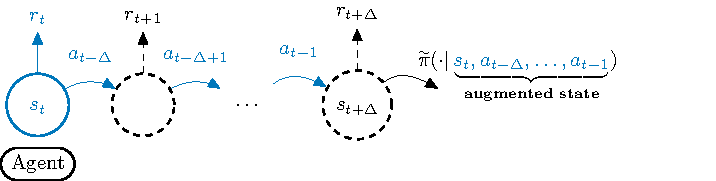
\includegraphics[bylabel=counterexamplemtmdp]{img/thesis_plots.pdf}
    \caption{Counter example for the conjecture that the higher the mean delay, the lower the performance. 
    The agent has two actions, $a$ and $b$, in each of the two states. The agent has, whatever the action, whatever the state, $1/2$ probability to transition to the other state and $1/2$ to remain in the same state. The reward is $r(s_1,b)=r(s_0,a)=1$ and $r(s_0,b)=r(s_1,a)=0$. The reward and transition function are specially defined such two agents, one with a smaller expected delay but less mass on the undelayed weight $\lambda_0$ compared to the other, will perform worse.}
    \label{fig:counter_example_mtmdp}
\end{figure}


Therefore, we need to find another way to compare two delay vectors. A way to consider the distribution of $\boldsymbol\lambda$ as a whole would be to consider its cumulative distribution. 
It is the subject of the following conjecture.

\begin{conj}
\label{conj:delay_cumulativ_distrib}
    Let $\boldsymbol\lambda$ and $\boldsymbol\lambda'$, be two delay vectors. 
    Denote $F_{\boldsymbol\lambda}$ and $F_{\boldsymbol\lambda}'$ their respective cumulative distribution as represented in \Cref{fig:hist_delay}.
    If, for any $i\in\naturalnumbers$:
    \begin{align*}
        F_{\boldsymbol\lambda}(i) \ge F_{\boldsymbol\lambda}'(i),
    \end{align*}
    then their optimal expected discounted return and average reward satisfy,
    \begin{align*}
        &\expectedreturn[\gamma][\star](\boldsymbol\lambda) \ge        \expectedreturn[\gamma][\star](\boldsymbol\lambda') 
        \\
        &\averagereturnfunction[\star](\boldsymbol\lambda)\ge\averagereturnfunction[\star](\boldsymbol\lambda').
    \end{align*}
\end{conj}

\begin{figure}[t]
    \centering
    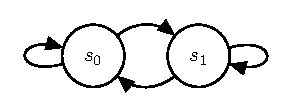
\includegraphics[labelmtd=histogramdelayvector]{img/thesis_plots_mtd.pdf}
    \caption{Example of delay vector $\boldsymbol\lambda$ with associated cumulative distribution function. The weight $\lambda_i$ is associated to delay $i$.}
    \label{fig:hist_delay}
\end{figure}

As an argument for the conjecture, we provide the following idea. 
Let $\delayedmarkovdecisionprocess$ and $\delayedmarkovdecisionprocess'$ be two \glspl{ismmdp} with respective delay vectors $\boldsymbol\lambda$ and $\boldsymbol\lambda'$.
Assume that $\forall i\in\naturalnumbers, F_{\boldsymbol\lambda}(i) \ge F_{\boldsymbol\lambda}'(i)$ and that $\boldsymbol\lambda$ has all its weight in $\lambda_\delay$ for $\delay\in[\![0,\delaymax]\!]$. 
For a policy $\delayedpolicy'$, an augmented state $x_t=(s_t,a_{t-\delaymax},\dots,a_{t-1})$ and an action $a_{t}\sim\delayedpolicy'$, a new state of the underlying \gls{mdp} is sampled in $\delayedmarkovdecisionprocess'$ under the distribution,
\begin{align}
    s_{t+1}\sim p(\cdot\vert x_t,a_{t})= \sum_{g=\delay}^{\delaymax'}\lambda_g' \transitionfunction(\cdot\vert s_t,a_{t-g}).\label{eq:proba_trans_plus_delayed}
\end{align}
Note that the summation starts at $\delay$ since $\forall i\in\naturalnumbers, F_{\boldsymbol\lambda}(i) \ge F_{\boldsymbol\lambda}'(i)$ and $\boldsymbol\lambda$ has all its weight on $\lambda_\delay$.
In $\delayedmarkovdecisionprocess$, the action selected by the agent at time $t$ will be applied exactly at time $t+\delay$.
One could therefore build a policy $\delayedpolicy$ in $\delayedmarkovdecisionprocess$ such the action it had selected at time $t-\delay$ exactly reproduces the probability of \Cref{eq:proba_trans_plus_delayed}. 
Formally, this would be the case if,
\begin{align*}
    \delayedpolicy(a\vert x_{t-\delay}) = \sum_{g=\delay}^{\delaymax'}\lambda_g'  \delta_{a_{t-g}}(a).
\end{align*}
Therefore, this agent would populate its augmented state with actions sampled from a different distribution than $\delayedpolicy'$.
However, if $\delayedpolicy$ is history-based, it can keep a memory of the actions that $\delayedpolicy'$  would have in its buffer. 
Yet, a technical complexity lies in the initialisation of the processes. 
If $\delayedmarkovdecisionprocess$ and $\delayedmarkovdecisionprocess'$ start with the same sequence of actions in their buffer, due to their different delay vectors, the first states in $\statespace$ will be sampled from different distributions, while the agent will have no control on it.

In the following, we continue to study the impact of the delay by evaluating its effect on the variance.
We show that not only does the performance decrease as the delay increases, but also the variance of the expected return or average reward shrinks. 
This result applies to constantly delayed \gls{dmdp}. 

\begin{prop}
\label{pp:var_ismmdp}
    Let $\delayedmarkovdecisionprocess_{1}$ and $\delayedmarkovdecisionprocess_{2}$ be two consistent \glspl{dmdp} with respective constant delay $\delay_1$ and $\delay_2$ and augmented state spaces $\augmentedstatespace_1$ and $\augmentedstatespace_2$. 
    Assume $\delay_1<\delay_2$.
    Consider $\delayedpolicy_2$ a policy for $\delayedmarkovdecisionprocess_{2}$ with $\sigma$-finite occupancy measure.
    Then, there exists a policy $\delayedpolicy_1$ for $\delayedmarkovdecisionprocess_{1}$ such that, $\forall x_1\in\augmentedstatespace_1$,
    $\mathbb{E}^{\delayedpolicy_1}[Y\vert
    x_1]=\mathbb{E}^{\delayedpolicy_2}[Y\vert x_1]$ and,
    \begin{align*}
         \mathbb{V}\mathrm{ar}^{\delayedpolicy_2}\left[\mathbb{E}^{\delayedpolicy_2}[Y\vert a,x_2]\right]\le\mathbb{V}\mathrm{ar}^{\delayedpolicy_1}\left[\mathbb{E}^{\delayedpolicy_1}[Y\vert a,x_1]\right],
    \end{align*}
    where $x_2\in\augmentedstatespace_2$ is the augmented state built from $x_1$ and $Y$ is a random variable that denotes expected discounted returns with either infinite horizon or average reward. 
    The term $\mathbb{E}^{\pi}[Y\vert a,x]$ is the conditional expectation of $Y$ under policy $\pi$ starting from the augmented state $x$ and selecting action $a$ first while $\mathbb{V}\mathrm{ar}^{\pi}$ denotes the variance under the state-action distribution induced by policy $\pi$.
\end{prop}
\begin{proof}
    Recall the law of total variance; for some random variables $X$ and $Y$ such that $Y$ has finite variance, one has
    \begin{align*}
        \variance[Y] = \expectedvalue\left[\variance[Y\vert X]\right] + \variance\left[\expectedvalue[Y\vert X]\right].
    \end{align*}
    We will apply this result to $\textstyle Y=\sum_{t=0}^\infty \gamma^{t} r(s_{t},a_{t})$ in the case of expected return or $\textstyle Y=\frac{1}{H}\sum_{t=0}^\infty r(s_{t},a_{t})$ in the case of average reward\footnote{Since the proof is similar in both cases, we do not make a difference in the notation.}.
    Note that, by the assumption of a bounded reward ($0\le r(s,a)\le \maximumreward$), $Y$ has a finite variance. 
    Now, let $\delayedpolicy_2$ be a policy in $\delayedmarkovdecisionprocess_{2}$ with $\sigma$-finite occupancy measure.
    By \Cref{corol:markov_optimal_delayed_equiv}, there exists a Markovian policy in $\delayedmarkovdecisionprocess_{1}$ with the same state occupancy measure in $\augmentedstatespace_1\times\actionspace$ as  $\delayedpolicy_2$.
    By \cite[Lemma~1]{laroche2022non} they have the same expected return or average reward.
    This shows that $\mathbb{E}^{\delayedpolicy_1}[Y]=\mathbb{E}^{\delayedpolicy_2}[Y]$ and, in particular, for an action $a\in\actionspace$ and an augmented state $x_2\in\augmentedstatespace_2$, $\mathbb{E}^{\delayedpolicy_1}[Y\vert a,x_2]=\mathbb{E}^{\delayedpolicy_2}[Y\vert a,x_2]$.
    Now, recall also that, given two random variables $X_1$ and $X_2$, one has,
    \begin{align*}
        \variance\left[\expectedvalue[Y\vert X_1]\right]\le \variance\left[\expectedvalue[Y\vert X_1,X_2]\right].
    \end{align*}
    Therefore, if we also note $x_1\in\augmentedstatespace_1$ the current augmented state in $\delayedmarkovdecisionprocess_1$, one has,
    \begin{align*}
        \mathbb{V}\mathrm{ar}^{\delayedpolicy_2}\left[\mathbb{E}^{\delayedpolicy_2}[Y\vert a,x_2]\right] &\le \mathbb{V}\mathrm{ar}^{\delayedpolicy_2}\left[\mathbb{E}^{\delayedpolicy_2}[Y\vert a,x_2,x_1]\right]
        \\
        &=\mathbb{V}\mathrm{ar}^{\delayedpolicy_2}\left[\mathbb{E}^{\delayedpolicy_2}[Y\vert a,x_1]\right],
    \end{align*}
    where we note that $Y$ depends only on future rewards and $x_1$ contains more recent information than $x_2$ since $\delay_1<\delay_2$. 
    The last equation holds by the Markovianity of the underlying process. 
    Next, we express the last term of the above equation under the distribution induced by $\delayedpolicy_1$,
    \begin{align}
        \mathbb{V}\mathrm{ar}^{\delayedpolicy_2}\left[\mathbb{E}^{\delayedpolicy_2}[Y\vert a,x_1]\right] 
        &= \mathbb{V}\mathrm{ar}^{\delayedpolicy_2}\left[\mathbb{E}^{\delayedpolicy_1}[Y\vert a,x_1]\right]\label{eq:same_return_f}
        \\
        &= \mathbb{V}\mathrm{ar}^{\delayedpolicy_1}\left[\mathbb{E}^{\delayedpolicy_1}[Y\vert a,x_1]\right]\label{eq:same_distrib_f},
    \end{align}
    where \Cref{eq:same_return_f} holds since the policies have the same return and \Cref{eq:same_distrib_f} since the policies have the same state occupancy measure on $\augmentedstatespace_1\times\actionspace$. 
    Regrouping the two equations yields the result.
\end{proof}

This result shows that the higher the delay, the less control the agent has and the lower the variance of its return is. 
The range of returns that a delayed policy can get shrinks as the delay increases.
In the limit, when the delay grows to infinity, the agent no longer has control over the sequence of actions, and the expected return or average reward follows the stochastic of the \gls{mdp} only. 

We can also easily extend \Cref{th:perf_delay_vector_all_weight} to show that the worst delayed policy is better than the worst undelayed policy.

\begin{coroll}[Corollary of \Cref{th:perf_delay_vector_all_weight}]
\label{th:inverse_perf_delay_vector_all_weight}
    Let $\delayedmarkovdecisionprocess_{1}$ and $\delayedmarkovdecisionprocess_{2}$ be two consistent \glspl{dmdp} with respective constant delay $\delay_1$ and $\delay_2$.
    Consider $\expectedreturn[1][W]$ and $\expectedreturn[2][W]$, the worst expected discounted returns with infinite horizon or average reward obtained over the set of delayed policies.
    If $\delay_1<\delay_2$, then one has:
    \begin{align*}
        \expectedreturn[1][W] \le \expectedreturn[2][W].
    \end{align*}
\end{coroll}
\begin{proof}
    It suffices to apply \Cref{th:perf_delay_vector_all_weight} to the process in which the reward function is replaced by its additive inverse.
\end{proof}

Therefore, the range of returns that are attainable by the set of delayed policies shrinks as the delay increases.
In the limit, when the delay grows to infinity, all policies yield the same expected return or average reward.

The last two results combined give us more understanding of the problem of delayed \gls{rl}. 
The longer the delay, the less the environment is controllable, and the smallest the range of possible returns. 
This phenomenon is represented in \Cref{fig:evolution_delay}.

\begin{figure}[t]
    \centering
    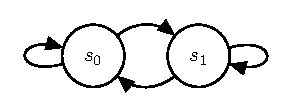
\includegraphics[labelmtd=policyreturn]{img/thesis_plots_mtd.pdf}
    \caption{A representation of the theoretical insights for the performance of delayed policies. 
    The x-axis is an abstract quantity representing the state distribution attained by a given policy while the y-axis shows the performance of that policy.
    The outer ellipse represents the set of all random history-based and undelayed policies. 
    The optimal undelayed policy would be the uppermost point of this ellipse.
    As the delays $\delay$ grows, the set of attainable returns and state distributions contracts until the delay becomes infinite, at which point the agent loses all control.}
    \label{fig:evolution_delay}
\end{figure}





\subsection{Learning in an ISM-MDP}

\glspl{ismmdp}, when seen as \glspl{mdp} by augmentation of the state, have a particular structure that we will study in this section, in order to understand which algorithms from the literature may apply to them. 

First, a problematic result is that \glspl{ismmdp} are generally not \emph{unichain}, even though the underlying \gls{mdp} is. An \gls{mdp} is unichain when the transition matrix of any stationary and deterministic policy is unichain \cite[Section~8.3.1]{puterman1994markov} (see also \Cref{def:unichain_mc}). 
In this section, when referring to \glspl{ismmdp}, we intend for the \gls{mdp} to which they can be cast following \Cref{prop:equ_mdp_is_mtdmdp}.

\begin{prop}
\label{pp:unichain_ismmdp}
    There exist \glspl{ismmdp} that are not unichain even though the underlying \gls{mdp} is.
\end{prop}
\begin{proof}
    In an \gls{ismmdp} built on top of a unichain \gls{mdp}, consider some deterministic stationary policy $\pi$  which given an augmented state $x=(s,a_1,\dots,a_\delay)$ reads:
    \begin{align*}
        \pi(x) = a_\delay.
    \end{align*}
    Then, this policy induces exactly $\cardinal{\actionspace}$ chains on $\augmentedstatespace$.
\end{proof}


\begin{remark}
    The policy defined in the previous proof visits all states $s\in\statespace$ since the underlying \gls{mdp} is unichain, and the policy $\pi(s) = a$ is deterministic and stationary. 
    However, it does not visit all the augmented states in $\augmentedstatespace$.
\end{remark}

The previous result means that some algorithms, such as UCRL~\cite{auer2006logarithmic} cannot be applied directly to \glspl{ismmdp} with augmented states.
A more promising road is the one of UCRL2~\cite{auer2008near} which applies to \emph{communicating} \glspl{mdp} \cite[Section~8.3.1]{puterman1994markov} (see also \Cref{def:communicating_mdp}).

\begin{prop}[Communicating ISM-MDP]
\label{pp:communicating_ismmdp}
    Consider a communicating \gls{mdp} $\markovdecisionprocess$ and an \gls{ismmdp} $\delayedmarkovdecisionprocess_{\boldsymbol\lambda}$ built upon it. 
    Then, the \gls{ismmdp} is communicating as well.
\end{prop}
\begin{proof}
    We first prove the result for constantly delayed \gls{dmdp}, before proving the generalisation to \gls{ismmdp}.
    
    For a delayed policy $\delayedpolicy$, we note $(p^\delayedpolicy)^{(k)}(s'\vert x)$ the probability that the state of the environment is $s'$ after applying the $k$ oldest actions of the augmented state starting from the state $s$ in $x$.
    If $k>\delaymax$, then the successive actions are sampled by $\delayedpolicy$. 
    Similarly, for an undelayed policy $\pi$,  we note $(p^\pi)^{(k)}(s'\vert s)$ the probability that the state of the environment is $s'$ after following policy $\pi$ for $k$ steps, starting from $s$.
    
    Let $x=(s,a_1,\dots,a_\delay)$ and $x'=(s',a_1',\dots,a_\delay')$ be two augmented states for $\delayedmarkovdecisionprocess_{\boldsymbol\lambda}$.
    Let $s''\in\statespace$ such that $(p^\delayedpolicy)^{(\delaymax)}(s''\cdot x)>0$. 
    Since the underlying \gls{mdp} is communicating, there exists an undelayed policy $\pi\in\Pi^{\text{SD}}$ and $k\in\naturalnumbers$ such that $(p^\pi)^{(k)}(s'\vert s'')>0$. 
    Let $k$ be the smallest such number.  
    Let us now note $\tau$ a trajectory in the undelayed \gls{mdp} that goes from $s$ to $s''$ in $\delaymax$ steps first, then from $s''$ to $s'$ in $k$ steps with probability $p^\pi(\tau)>0$. 
    The aforementioned properties guarantee that such a trajectory exists. 
    Specifically, we note,
    \begin{align*}
        \tau=(s,a_0^\star,s_1^\star,a_1^\star,\dots,a_{\delaymax-1}^\star,s'',a_{\delaymax}^\star,\dots,s_{k+\delaymax-1}^\star,a_{k+\delaymax-1}^\star,s').
    \end{align*}
    We can rewrite $s$ as $s_0^\star$ and $s''$ as $s_{\delaymax}^\star$ and for the action contained in $x'$, we note $a_i'$ as $a_{k+\delaymax+i-1}^\star$. 
    We are now ready to define a candidate stationary deterministic delayed policy $\delayedpolicy$ to take us from $s$ to $s'$ with non-zero probability. 
    By defining $x_i^\star=(s_i^\star,a_i^\star,\dots,a_{i+\delaymax-1}^\star)$, the policy is defined as follows,
    \begin{align*}
        &\delayedpolicy(x_i^\star) = a_{i+\delaymax}^\star.
    \end{align*}
    The definition for other augmented states is irrelevant and can be made freely.
    This policy has a non-zero probability to go from $x$ to $x'$ but it is not clear whether it actually defines a policy.
    Indeed, the agent could be faced twice with the same augmented state while the above policy would indicate two different actions. 
    Said alternatively, $\delayedpolicy$ may not be a correctly defined function. 
    We shall now demonstrate that this is not the case, or when it is, a simple modification can be applied. 
    
    Let $i,j\in\naturalnumbers$ such that $\delaymax<i<j$ and  $x_i^\star=x_j^\star$ but $\delayedpolicy(x_i^\star)\neq \delayedpolicy(x_j^\star)$.
    Then, the trajectory that goes from $s_j^\star$ to $s$ is long $\delaymax+k-j<\delaymax+k-i$ but $s_j^\star=s_i^\star$ so the undelayed policy as defined after time $j$ could be applied at time $i$ to yield a shorter trajectory with strictly positive probability. This contradicts the assumption on $\tau$.
    There remains a little complexity; as the reader noticed, we assumed $\delaymax<i<j$.
    Indeed, since we do not control for the first $\delaymax$ actions, an augmented state present after the $\delaymax$ step may already be found in the first $\delaymax$ steps.
    However, this acts as if the agent were already in a more advanced part of the trajectory $\tau$, therefore, one can keep the action defined for the augmented state with the higher index as the value for $\delayedpolicy$.
    This ensures that $\delayedpolicy$ is a properly defined stationary deterministic policy that verifies $(p^\delayedpolicy)^{(\delaymax+k)}(x'\vert x)>0$. 
    The \gls{dmdp} is therefore communicating.
    
    The result for \gls{ismmdp} is obtained as follows.
    At any step, there is a non-zero probability that the action at the $\delaymax$ position is executed; therefore, there is a non-zero probability that a trajectory is sampled as if the whole process were a $\delaymax$-constantly delayed \gls{dmdp}.
    From the above, because the latter is communicating, there is therefore a non-zero probability of reaching $x'$ starting from $x$ in the original \gls{ismmdp}.
\end{proof}

\begin{remark}
    This result, as shown in the proof and because \glspl{ismmdp} includes constantly delayed \glspl{dmdp} as a special case, demonstrates that a constantly delayed \gls{dmdp} is communicating if the underlying \gls{mdp} is.
\end{remark}

With this property, one can therefore apply UCRL2~\cite{auer2008near} to learn a policy in an \gls{ismmdp}.
As said in \Cref{subsec:theoretical_rl}, the regret of UCRL2 depends on the notion of the diameter of the \gls{mdp}, defined in \Cref{def:diameter}.
The diameter in an \gls{ismmdp} is obviously lower bounded by the diameter of the underlying \gls{mdp}.
One can give a better lower bound on the diameter by applying a result by \cite{auer2008near} to this special case. 

\begin{prop}
    Let $\delayedmarkovdecisionprocess_{\boldsymbol\lambda}$ be an \gls{ismmdp} with maximum delay $\delaymax$ and such that its action space consists of two actions or more, then
    \begin{align*}
        D(\delayedmarkovdecisionprocess_{\boldsymbol\lambda})\geq \delaymax-3 + \log_{\cardinal{\actionspace}}\cardinal{\statespace}
    \end{align*}
\end{prop}
\begin{proof}
    From \cite[Corollary~15]{auer2008near}, we know that, for some \gls{mdp} $\markovdecisionprocess$ with state space $\statespace$ and action space $\actionspace$,
    \begin{align*}
        D(\markovdecisionprocess)\ge\log_{\cardinal{\actionspace}}\cardinal{\statespace}-3.
    \end{align*}
    Applying this result to the augmented \gls{mdp} obtained from \gls{ismmdp} with state space $\statespace\times\actionspace^{\delaymax}$ concludes the proof. 
\end{proof}

We see here the additive impact of the delay on the diameter. Note that, even if the term $-3 + \log_{\cardinal{\actionspace}}\cardinal{\statespace}$ happened to be negative, the diameter can never be inferior to $\delaymax$. To show this, it suffices to consider two augmented states whose actions do not match, it obviously takes more than $\delaymax$ actions to take from one to the other. 